\chapter{Introduction}
\label{chap:introduction}

\section{Overall description}
The goal of this project is catching a ping pong ball released above a platform, on which three piezoelectric elements are placed in a triangular pattern as shown in Figure \ref{fig:sideview}. Once the ball has hit the platform once, each of the piezo elements will generate a signal and permit triangulation of the impact point. When the impact point has been found, a net will catch the ball when it returns toward the platform after the first bounce.

\begin{figure}[htb]
	\centering
	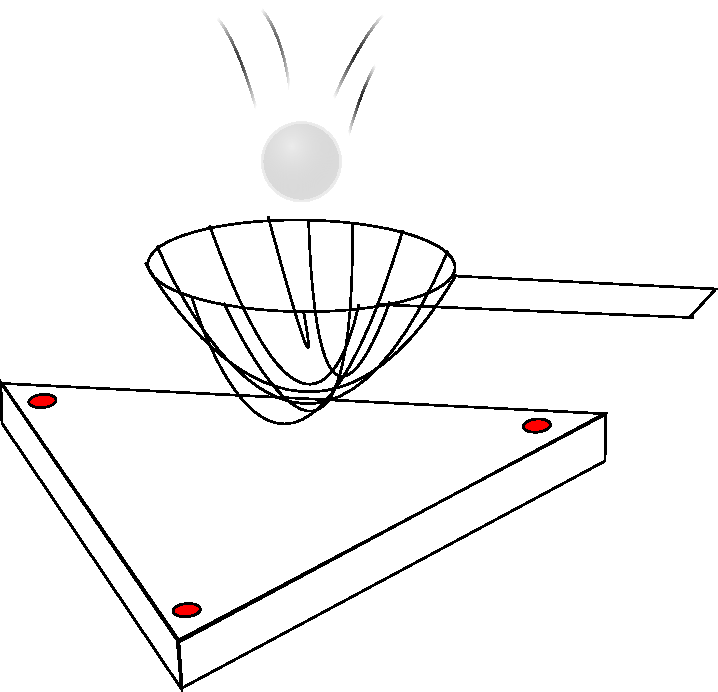
\includegraphics[width=0.8\textwidth]{figures/sideview}
	\caption{Side view of the platform surface area and the net. The red markings are piezoelectric sensors.}
	\label{fig:sideview}
\end{figure}

Overall the different tasks of the project are thus:
\begin{itemize}
	\item Calculating the xy-coordinate of the impact point
	\item Calculating the hight the ball will bounce back to
	\item Moving an arm -- holding a net -- to catch the ball after it has bounced once
\end{itemize}

\subsection{Report structure}
The report is organized so it starts with the explanation of the project's methodology  and the equipment used (\ref{chap:methodology}), followed by the description of the design and implementation of the Main PCB (\ref{chap:main_board}) and the Control-Brick-Sorter Module PCB (\ref{chap:bricksorter}) along with the FPGA's programming work (\ref{chap:fpga}) and the PC program (\ref{chap:pc_program}) developed and used as an interface between the FPGA to finish with the conclusions and the goals achieved (\ref{chap:conclusions}).